\documentclass[12pt,journal,compsoc]{IEEEtran}

% For Computer Society journals, IEEEtran defaults to the use of 
% Palatino/Palladio as is done in IEEE Computer Society journals.
% To go back to Times Roman, you can use this code:
%\renewcommand{\rmdefault}{ptm}\selectfont



% *** CITATION PACKAGES ***
%
\ifCLASSOPTIONcompsoc
  % IEEE Computer Society needs nocompress option
  % requires cite.sty v4.0 or later (November 2003)
  % \usepackage[nocompress]{cite}
\else
  % normal IEEE
  % \usepackage{cite}
\fi

% *** GRAPHICS RELATED PACKAGES ***
%
\ifCLASSINFOpdf
  % \usepackage[pdftex]{graphicx}
  % declare the path(s) where your graphic files are
  % \graphicspath{{../pdf/}{../jpeg/}}
  % and their extensions so you won't have to specify these with
  % every instance of \includegraphics
  % \DeclareGraphicsExtensions{.pdf,.jpeg,.png}
\else
  % or other class option (dvipsone, dvipdf, if not using dvips). graphicx
  % will default to the driver specified in the system graphics.cfg if no
  % driver is specified.
  % \usepackage[dvips]{graphicx}
  % declare the path(s) where your graphic files are
  % \graphicspath{{../eps/}}
  % and their extensions so you won't have to specify these with
  % every instance of \includegraphics
  % \DeclareGraphicsExtensions{.eps}
\fi

% *** MATH PACKAGES ***
%
%\usepackage[cmex10]{amsmath}
% A popular package from the American Mathematical Society that provides
% many useful and powerful commands for dealing with mathematics. If using
% it, be sure to load this package with the cmex10 option to ensure that
% only type 1 fonts will utilized at all point sizes. Without this option,
% it is possible that some math symbols, particularly those within
% footnotes, will be rendered in bitmap form which will result in a
% document that can not be IEEE Xplore compliant!
%
% Also, note that the amsmath package sets \interdisplaylinepenalty to 10000
% thus preventing page breaks from occurring within multiline equations. Use:
%\interdisplaylinepenalty=2500
% after loading amsmath to restore such page breaks as IEEEtran.cls normally
% does. amsmath.sty is already installed on most LaTeX systems. The latest
% version and documentation can be obtained at:
% http://www.ctan.org/tex-archive/macros/latex/required/amslatex/math/

% *** SPECIALIZED LIST PACKAGES ***
%\usepackage{acronym}
% acronym.sty was written by Tobias Oetiker. This package provides tools for
% managing documents with large numbers of acronyms. (You don't *have* to
% use this package - unless you have a lot of acronyms, you may feel that
% such package management of them is bit of an overkill.)
% Do note that the acronym environment (which lists acronyms) will have a
% problem when used under IEEEtran.cls because acronym.sty relies on the
% description list environment - which IEEEtran.cls has customized for
% producing IEEE style lists. A workaround is to declared the longest
% label width via the IEEEtran.cls \IEEEiedlistdecl global control:
%
% \renewcommand{\IEEEiedlistdecl}{\IEEEsetlabelwidth{SONET}}
% \begin{acronym}
%
% \end{acronym}
% \renewcommand{\IEEEiedlistdecl}{\relax}% remember to reset \IEEEiedlistdecl
%
% instead of using the acronym environment's optional argument.
% The latest version and documentation can be obtained at:
% http://www.ctan.org/tex-archive/macros/latex/contrib/acronym/


%\usepackage{algorithmic}
% algorithmic.sty was written by Peter Williams and Rogerio Brito.
% This package provides an algorithmic environment fo describing algorithms.
% You can use the algorithmic environment in-text or within a figure
% environment to provide for a floating algorithm. Do NOT use the algorithm
% floating environment provided by algorithm.sty (by the same authors) or
% algorithm2e.sty (by Christophe Fiorio) as IEEE does not use dedicated
% algorithm float types and packages that provide these will not provide
% correct IEEE style captions. The latest version and documentation of
% algorithmic.sty can be obtained at:
% http://www.ctan.org/tex-archive/macros/latex/contrib/algorithms/
% There is also a support site at:
% http://algorithms.berlios.de/index.html
% Also of interest may be the (relatively newer and more customizable)
% algorithmicx.sty package by Szasz Janos:
% http://www.ctan.org/tex-archive/macros/latex/contrib/algorithmicx/




% *** ALIGNMENT PACKAGES ***
%
%\usepackage{array}
% Frank Mittelbach's and David Carlisle's array.sty patches and improves
% the standard LaTeX2e array and tabular environments to provide better
% appearance and additional user controls. As the default LaTeX2e table
% generation code is lacking to the point of almost being broken with
% respect to the quality of the end results, all users are strongly
% advised to use an enhanced (at the very least that provided by array.sty)
% set of table tools. array.sty is already installed on most systems. The
% latest version and documentation can be obtained at:
% http://www.ctan.org/tex-archive/macros/latex/required/tools/


%\usepackage{mdwmath}
%\usepackage{mdwtab}
% Also highly recommended is Mark Wooding's extremely powerful MDW tools,
% especially mdwmath.sty and mdwtab.sty which are used to format equations
% and tables, respectively. The MDWtools set is already installed on most
% LaTeX systems. The lastest version and documentation is available at:
% http://www.ctan.org/tex-archive/macros/latex/contrib/mdwtools/


% IEEEtran contains the IEEEeqnarray family of commands that can be used to
% generate multiline equations as well as matrices, tables, etc., of high
% quality.


%\usepackage{eqparbox}
% Also of notable interest is Scott Pakin's eqparbox package for creating
% (automatically sized) equal width boxes - aka "natural width parboxes".
% Available at:
% http://www.ctan.org/tex-archive/macros/latex/contrib/eqparbox/




% *** SUBFIGURE PACKAGES ***
%\ifCLASSOPTIONcompsoc
%  \usepackage[caption=false,font=normalsize,labelfont=sf,textfont=sf]{subfig}
%\else
%  \usepackage[caption=false,font=footnotesize]{subfig}
%\fi
% subfig.sty, written by Steven Douglas Cochran, is the modern replacement
% for subfigure.sty, the latter of which is no longer maintained and is
% incompatible with some LaTeX packages including fixltx2e. However,
% subfig.sty requires and automatically loads Axel Sommerfeldt's caption.sty
% which will override IEEEtran.cls' handling of captions and this will result
% in non-IEEE style figure/table captions. To prevent this problem, be sure
% and invoke subfig.sty's "caption=false" package option (available since
% subfig.sty version 1.3, 2005/06/28) as this is will preserve IEEEtran.cls
% handling of captions.
% Note that the Computer Society format requires a larger sans serif font
% than the serif footnote size font used in traditional IEEE formatting
% and thus the need to invoke different subfig.sty package options depending
% on whether compsoc mode has been enabled.
%
% The latest version and documentation of subfig.sty can be obtained at:
% http://www.ctan.org/tex-archive/macros/latex/contrib/subfig/




% *** FLOAT PACKAGES ***
%
%\usepackage{fixltx2e}
% fixltx2e, the successor to the earlier fix2col.sty, was written by
% Frank Mittelbach and David Carlisle. This package corrects a few problems
% in the LaTeX2e kernel, the most notable of which is that in current
% LaTeX2e releases, the ordering of single and double column floats is not
% guaranteed to be preserved. Thus, an unpatched LaTeX2e can allow a
% single column figure to be placed prior to an earlier double column
% figure. The latest version and documentation can be found at:
% http://www.ctan.org/tex-archive/macros/latex/base/


%\usepackage{stfloats}
% stfloats.sty was written by Sigitas Tolusis. This package gives LaTeX2e
% the ability to do double column floats at the bottom of the page as well
% as the top. (e.g., "\begin{figure*}[!b]" is not normally possible in
% LaTeX2e). It also provides a command:
%\fnbelowfloat
% to enable the placement of footnotes below bottom floats (the standard
% LaTeX2e kernel puts them above bottom floats). This is an invasive package
% which rewrites many portions of the LaTeX2e float routines. It may not work
% with other packages that modify the LaTeX2e float routines. The latest
% version and documentation can be obtained at:
% http://www.ctan.org/tex-archive/macros/latex/contrib/sttools/
% Do not use the stfloats baselinefloat ability as IEEE does not allow
% \baselineskip to stretch. Authors submitting work to the IEEE should note
% that IEEE rarely uses double column equations and that authors should try
% to avoid such use. Do not be tempted to use the cuted.sty or midfloat.sty
% packages (also by Sigitas Tolusis) as IEEE does not format its papers in
% such ways.
% Do not attempt to use stfloats with fixltx2e as they are incompatible.
% Instead, use Morten Hogholm'a dblfloatfix which combines the features
% of both fixltx2e and stfloats:
%
% \usepackage{dblfloatfix}
% The latest version can be found at:
% http://www.ctan.org/tex-archive/macros/latex/contrib/dblfloatfix/


%\ifCLASSOPTIONcaptionsoff
%  \usepackage[nomarkers]{endfloat}
% \let\MYoriglatexcaption\caption
% \renewcommand{\caption}[2][\relax]{\MYoriglatexcaption[#2]{#2}}
%\fi
% endfloat.sty was written by James Darrell McCauley, Jeff Goldberg and 
% Axel Sommerfeldt. This package may be useful when used in conjunction with 
% IEEEtran.cls'  captionsoff option. Some IEEE journals/societies require that
% submissions have lists of figures/tables at the end of the paper and that
% figures/tables without any captions are placed on a page by themselves at
% the end of the document. If needed, the draftcls IEEEtran class option or
% \CLASSINPUTbaselinestretch interface can be used to increase the line
% spacing as well. Be sure and use the nomarkers option of endfloat to
% prevent endfloat from "marking" where the figures would have been placed
% in the text. The two hack lines of code above are a slight modification of
% that suggested by in the endfloat docs (section 8.4.1) to ensure that
% the full captions always appear in the list of figures/tables - even if
% the user used the short optional argument of \caption[]{}.
% IEEE papers do not typically make use of \caption[]'s optional argument,
% so this should not be an issue. A similar trick can be used to disable
% captions of packages such as subfig.sty that lack options to turn off
% the subcaptions:
% For subfig.sty:
% \let\MYorigsubfloat\subfloat
% \renewcommand{\subfloat}[2][\relax]{\MYorigsubfloat[]{#2}}
% However, the above trick will not work if both optional arguments of
% the \subfloat command are used. Furthermore, there needs to be a
% description of each subfigure *somewhere* and endfloat does not add
% subfigure captions to its list of figures. Thus, the best approach is to
% avoid the use of subfigure captions (many IEEE journals avoid them anyway)
% and instead reference/explain all the subfigures within the main caption.
% The latest version of endfloat.sty and its documentation can obtained at:
% http://www.ctan.org/tex-archive/macros/latex/contrib/endfloat/
%
% The IEEEtran \ifCLASSOPTIONcaptionsoff conditional can also be used
% later in the document, say, to conditionally put the References on a 
% page by themselves.





% *** PDF, URL AND HYPERLINK PACKAGES ***
%
%\usepackage{url}
% url.sty was written by Donald Arseneau. It provides better support for
% handling and breaking URLs. url.sty is already installed on most LaTeX
% systems. The latest version and documentation can be obtained at:
% http://www.ctan.org/tex-archive/macros/latex/contrib/url/
% Basically, \url{my_url_here}.


% NOTE: PDF thumbnail features are not required in IEEE papers
%       and their use requires extra complexity and work.
%\ifCLASSINFOpdf
%  \usepackage[pdftex]{thumbpdf}
%\else
%  \usepackage[dvips]{thumbpdf}
%\fi
% thumbpdf.sty and its companion Perl utility were written by Heiko Oberdiek.
% It allows the user a way to produce PDF documents that contain fancy
% thumbnail images of each of the pages (which tools like acrobat reader can
% utilize). This is possible even when using dvi->ps->pdf workflow if the
% correct thumbpdf driver options are used. thumbpdf.sty incorporates the
% file containing the PDF thumbnail information (filename.tpm is used with
% dvips, filename.tpt is used with pdftex, where filename is the base name of
% your tex document) into the final ps or pdf output document. An external
% utility, the thumbpdf *Perl script* is needed to make these .tpm or .tpt
% thumbnail files from a .ps or .pdf version of the document (which obviously
% does not yet contain pdf thumbnails). Thus, one does a:
% 
% thumbpdf filename.pdf 
%
% to make a filename.tpt, and:
%
% thumbpdf --mode dvips filename.ps
%
% to make a filename.tpm which will then be loaded into the document by
% thumbpdf.sty the NEXT time the document is compiled (by pdflatex or
% latex->dvips->ps2pdf). Users must be careful to regenerate the .tpt and/or
% .tpm files if the main document changes and then to recompile the
% document to incorporate the revised thumbnails to ensure that thumbnails
% match the actual pages. It is easy to forget to do this!
% 
% Unix systems come with a Perl interpreter. However, MS Windows users
% will usually have to install a Perl interpreter so that the thumbpdf
% script can be run. The Ghostscript PS/PDF interpreter is also required.
% See the thumbpdf docs for details. The latest version and documentation
% can be obtained at.
% http://www.ctan.org/tex-archive/support/thumbpdf/


% NOTE: PDF hyperlink and bookmark features are not required in IEEE
%       papers and their use requires extra complexity and work.
% *** IF USING HYPERREF BE SURE AND CHANGE THE EXAMPLE PDF ***
% *** TITLE/SUBJECT/AUTHOR/KEYWORDS INFO BELOW!!           ***
\newcommand\MYhyperrefoptions{bookmarks=true,bookmarksnumbered=true,
pdfpagemode={UseOutlines},plainpages=false,pdfpagelabels=true,
colorlinks=true,linkcolor={black},citecolor={black},urlcolor={black},
pdftitle={Bare Demo of IEEEtran.cls for Computer Society Journals},%<!CHANGE!
pdfsubject={Typesetting},%<!CHANGE!
pdfauthor={Michael D. Shell},%<!CHANGE!
pdfkeywords={Computer Society, IEEEtran, journal, LaTeX, paper,
             template}}%<^!CHANGE!
%\ifCLASSINFOpdf
%\usepackage[\MYhyperrefoptions,pdftex]{hyperref}
%\else
%\usepackage[\MYhyperrefoptions,breaklinks=true,dvips]{hyperref}
%\usepackage{breakurl}
%\fi
% One significant drawback of using hyperref under DVI output is that the
% LaTeX compiler cannot break URLs across lines or pages as can be done
% under pdfLaTeX's PDF output via the hyperref pdftex driver. This is
% probably the single most important capability distinction between the
% DVI and PDF output. Perhaps surprisingly, all the other PDF features
% (PDF bookmarks, thumbnails, etc.) can be preserved in
% .tex->.dvi->.ps->.pdf workflow if the respective packages/scripts are
% loaded/invoked with the correct driver options (dvips, etc.). 
% As most IEEE papers use URLs sparingly (mainly in the references), this
% may not be as big an issue as with other publications.
%
% That said, Vilar Camara Neto created his breakurl.sty package which
% permits hyperref to easily break URLs even in dvi mode.
% Note that breakurl, unlike most other packages, must be loaded
% AFTER hyperref. The latest version of breakurl and its documentation can
% be obtained at:
% http://www.ctan.org/tex-archive/macros/latex/contrib/breakurl/
% breakurl.sty is not for use under pdflatex pdf mode.
%
% The advanced features offer by hyperref.sty are not required for IEEE
% submission, so users should weigh these features against the added
% complexity of use.
% The package options above demonstrate how to enable PDF bookmarks
% (a type of table of contents viewable in Acrobat Reader) as well as
% PDF document information (title, subject, author and keywords) that is
% viewable in Acrobat reader's Document_Properties menu. PDF document
% information is also used extensively to automate the cataloging of PDF
% documents. The above set of options ensures that hyperlinks will not be
% colored in the text and thus will not be visible in the printed page,
% but will be active on "mouse over". USING COLORS OR OTHER HIGHLIGHTING
% OF HYPERLINKS CAN RESULT IN DOCUMENT REJECTION BY THE IEEE, especially if
% these appear on the "printed" page. IF IN DOUBT, ASK THE RELEVANT
% SUBMISSION EDITOR. You may need to add the option hypertexnames=false if
% you used duplicate equation numbers, etc., but this should not be needed
% in normal IEEE work.
% The latest version of hyperref and its documentation can be obtained at:
% http://www.ctan.org/tex-archive/macros/latex/contrib/hyperref/





% *** Do not adjust lengths that control margins, column widths, etc. ***
% *** Do not use packages that alter fonts (such as pslatex).         ***
% There should be no need to do such things with IEEEtran.cls V1.6 and later.
% (Unless specifically asked to do so by the journal or conference you plan
% to submit to, of course. )


% correct bad hyphenation here
\hyphenation{op-tical net-works semi-conduc-tor}
\usepackage{graphicx}
\graphicspath{ {images/} }
\usepackage{caption}
\usepackage{subcaption}

\begin{document}
\title{Image Processing for Discovering\\ the Rules of Video Games}

\author{Erik~Culberson,
        Neil~Ferman,
      and~Viljo~Wagner}

% make the title area
\maketitle

\section{Introduction}
There are many examples of machine learning algorithms being able to play video games when the algorithms are integrated directly within the game. This is a costly process and needs hours of development work as well as needing more access to resources such as the source code of the video game. This approach also gives algorithms more in-game knowledge than a normal player would have. By removing this advantage from the algorithms we will be able to see how well the algorithms can compare to human players given an equal playing field. General Video Game Playing AI is a little newer, but has been approached in \cite{2}. Given the same inputs as a human player, a screen image as an input and a set of key controls as output, can the algorithm discover the set of rules of the game as well as the rules of the game world?

\section{Problem}
Current research into artificial learning in games focus heavily on algorithms' ability to discover the optimal or fastest solution to the current level or problem. The algorithms are given the rules and knowledge of the game and the environment before hand. This forces the algorithm to only be able to be used for one specific game. To create a general algorithm that can play multiple games, the first step is to allow the algorithm to learn the rules of the game on its own. This paper focuses on the question of whether an AI can learn the rules of the game, including inputs, as well as rewards and penalties of certain actions, and discover goals using only screenshots taken as the game is played.

\section{Game and Emulator}
We chose to use Ms. Pac-Man as our test game for this project. We chose this game due to its simplistic nature in understanding the game by image, but complication in AI. Ms. Pac-Man is a game where you play as Ms. Pac-Man, a character inside of a maze. Your objective is to eat little dots called pellets inside of the maze. There are four ghosts within the maze who chase Ms. Pac-Man that you want to avoid. The four ghosts are different colors and behave in slightly different ways. What makes the AI of Ms. Pac-Man interesting is how the ghosts have an expected behavior, but also have a random chance of taking a random route instead of following their expected behavior \cite{3}. This makes the AI less predictable for a player (and indeed for an AI) to learn.

To run the game, and be able to connect it with our algorithms, we used an emulator called FCEUX. FCEUX is an emulator capable of running games designed to run on the Nintendo Entertainment System (NES). FCEUX has plugins that allow a user to run lua scripts through it. It also offers debugging tools like memory address lookup and emulation speed. This makes it an ideal candidate for teaching an AI to play Ms. Pac-Man.

\section{Approach}
Several different algorithms were needed to achieve our goal. We will break each overall algorithm into steps for the project and go into detail of how each algorithm works. The steps are as follows:\\
\textbf{Image Capture}: Capture images of the game as it is played, frame by frame.\\
\textbf{Image Recognition}: Convert the image into an array of colors and coordinates, and separate images by parts.\\
\textbf{Learning}: Pass the encoded images as well as a set of valid inputs into a learning algorithm, to be used to learn the rules of the game and update accordingly. We tried two different learning algorithms: QLearning, and NEAT.

\section{Bridge}
Our bridge script was used as a way to connect the chosen emulator (FCEUX) with our image capture script. The bridge script was written in lua, and uses lua sockets to communicate with our python image capturing script. The bridge script contains the following functions:\\
\textbf{Set input key}\\
\textbf{Get Inputs}\\
\textbf{Get Screen}\\
\textbf{Get Location}\\
\textbf{Get Points}\\
\textbf{Reset}\\
\textbf{Done (ONLY DEATH)}\\
\textbf{Skip Frame}\\
\textbf{Get Palet Count}

\section{Image Processing}
The image processing algorithm gets the image from the lua bridge and applies the following operations to identify object in an image and pass them on to the Q-Learning/NEAT algorithms.\\ \\
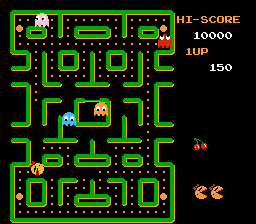
\includegraphics[scale=0.45]{frame626}

\textbf{Image to Image Delta:}
If the current image is not the first image processed, then the algorithm will compare the previous image to the current one and depending on the delta-score it will decide whether the current image is different enough to warrant a complete reprocessing of the current image or if it is sufficient to just process the regions of the image that have changed.

\textbf{Change Resolution:}
The resolution is being reduced to reduce the information density with the thought that only the most prominent features will be available afterwards. This works well for finding characters and objects in the image but most of the time any text based information like the score is lost.\\ \\
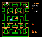
\includegraphics[scale=3]{6xdown}

\textbf{Convert to Grayscale:}
This steps helps improve the speed of the algorithm since the algorithm has to only deal with 8-bits of color instead of 24-bits. The grayscale conversion function can be provided with weight parameters for red, green and blue (RGB). This allows the highlighting of certain objects of interest.\\ \\
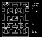
\includegraphics[scale=3]{gray}

\textbf{Neighbor-Matrix:}
The neighbor matrix is just there to determine which fields are of interest. For example when processing the first image there is only information on the part of the image that has been processed while further iterations have information on previous run throughs. The matrix is always relative to the pixel in the image that is being processed.

    The current Image Processing algorithm does no image classification but the algorithm has been set up in a way that it can be fed into a machine learning algorithm to optimize the weights for the different games that could be played, and then classify the different objects that are outputted.

\section{QLearning}
QLearning is an algorithm that uses Model-Based Learning. It was the first algorithm we tried to implement. It is an evolved form of Markov Chains. To summarize QLearning, it takes a state, and then has transitions from its current state into future states. Each transition has a probability of being taken to move into the next state. Each possible state that can be transitioned into (known as a future state) has a reward or penalty associated with it. QLearning will at first pick a future state at random, and then, based on whether a reward or penalty is reached, update the transition probability. What makes QLearning so appealing for learning games is that it can on occasion, take a route that seems sub-optimal to explore whether that future state (or any subsequent future state) might lead to greater rewards. This is good for games that have random chance outcomes that are sometimes bad, but sometimes good.
Our QLearning algorithm would take as input the boundaries of the screen, locations of enemy as well as Ms. Pac-Man, certain actions that gained rewards (increase score, eat pellets), and the state of Ms. Pac-Man (not dead, and dead). However, the QLearning did not seem to be very successful at learning the game. It mostly moved at random, and just oscillated back and forth between a couple of different hallways, and didn’t seek out pellets or avoid ghosts.

\section{NEAT (Neuro-Evolution Augmenting Topologies)}
Our NEAT algorithm was the second algorithm we tried but it did not fare better than Q-Learning. NEAT, better explained in the original paper \cite{8}, is a population of full neural networks that use a genetic algorithm to form the neural network structure and weights. This allows the algorithm to find a minimalist neural network that can complete the task at hand. 

For the NEAT algorithm are input was the image of the screen. Are image was 256x224 colored image which ment that we had to have 172,032 inputs to be able to hand the size of the image and the 3 RGB values per pixel. This was way to large for the NEAT alogrithm to handle to to reduce it we pixelated the image into a 28x32 image as shown in figure 1-4. By doing this we were able to reduce are input to 2,688 still taking into account the RGB values of each pixel. Are outputs to are neural network were the 4 inputs the game accepted Up, Down, Left, and Right.

\begin{figure}
\centering
\begin{minipage}{.25\textwidth}
  \centering
  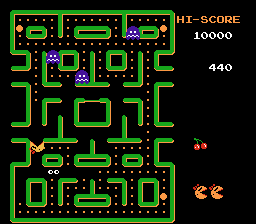
\includegraphics[width=.95\linewidth]{Original1.png}
  \captionof{figure}{Original}
  \label{fig:test1}
\end{minipage}%
\begin{minipage}{.25\textwidth}
  \centering
  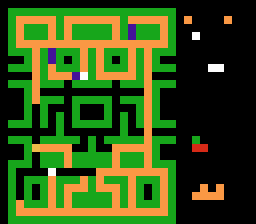
\includegraphics[width=.95\linewidth]{pixel1.png}
  \captionof{figure}{Pixelated}
  \label{fig:test2}
\end{minipage}
\end{figure}
\begin{figure}
\centering
\begin{minipage}{.25\textwidth}
  \centering
  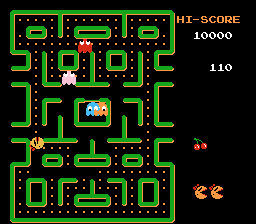
\includegraphics[width=.95\linewidth]{Original2.png}
  \captionof{figure}{Original}
  \label{fig:test1}
\end{minipage}%
\begin{minipage}{.25\textwidth}
  \centering
  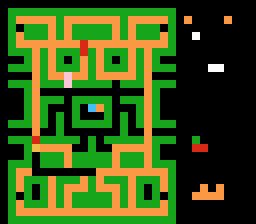
\includegraphics[width=.95\linewidth]{pixel2.png}
  \captionof{figure}{Pixelated}
  \label{fig:test2}
\end{minipage}
\end{figure}

We were not able to get this algorithm to work either and the reasons why we think the NEAT algorithm failed was, for two reasons, there are too many inputs or we did not give it enough time to train. Even though we reduced the inputs from are original 172,032 inputs to 2,688 inputs we did not take into account that because the NEAT algorithm starts off with 0 hidden nodes that it would take so long to generate a full connected graph that could take in all those inputs and create meaningful connection between all of the nodes. One solution to this is to do more image processing beforehand to find all the variables such as player position, enemy position, and so on to reduce the number of inputs which give the algorithm a chance to learn what the meaning behind the inputs are. 

Another solution would be to allow the algorithm to learn for a longer period of time. The NEAT algorithm ran for 121 generations with a population of 150. Over the 121 generations the best performing networks max fitness hovered around 39 points out of the total 177 points and did not show much improvement from generation to generation as shown in figure 5. Given more time for the algorithm to build a bigger graph or reducing the input we believe that the algorithm would be able to improve its fitness.

\begin{figure}
\centering
  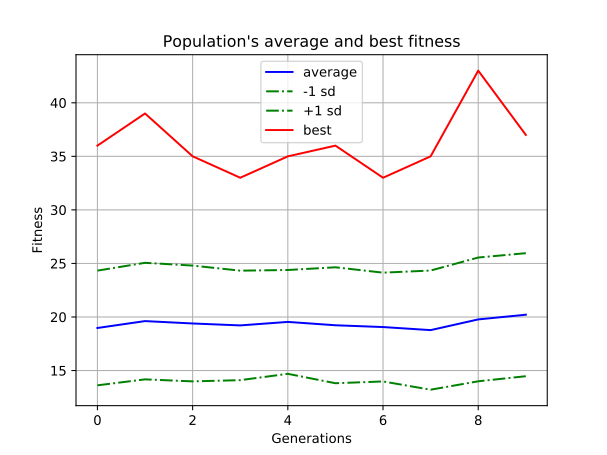
\includegraphics[width=1\linewidth]{avg_fitness.png}
\end{figure}

Another problem with our algorithm is that it took a very long time to learn. It took roughly 6 days to learn 121 generations. There are a couple of ways we think we can improve this time. The easiest being to introduce a timeout function that will fail the network after a set number of frames that have not added to the fitness of the network.

\section{Results}
We set out to create an algorithm that could learn and play virtually any game based on screenshots and learning inputs/rules of the game. The algorithms we came up with wound up having very limited capabilities. Currently the screen size of the game needs to be the same, and the game’s score needs to be provided to the algorithm so it can track rewards. We did not have enough time to really see how either QLearning or NEAT could really learn the rules of the game. Learning algorithms can take several days or weeks before real progress can be seen, and we have only been able to run it for a few days. The algorithm is able to learn to navigate the field after some time. However, learning past that (like, say, that eating blue ghosts can cause a reward) is unknown. A major limiting factor was that the Image Processing was literally just image processing which found objects based on given parameters but did no classification so the Q-Learning/NEAT algorithms had to figure out what the objects are by themselves. This is also why we decided to pull the position for the game character and the score from the Emulator RAM so we could at least start training the learning algorithms.

\section{What we learned and Future Ideas}
We had a lot of trouble connecting so many different, separate ideas, together. Especially connecting the image processing to our Learning algorithms was a big slow down for us. It is also not possible to get lua sockets on a Windows machine, a problem that prevented one of the researchers in improving QLearning, since he had Windows. There are better image processing libraries out there we would like to experiment with, such as Tensorflow. This could more readily solve the issue of classifying objects. NEAT and QLearning could both be greatly improved, as well as the inputs received by them could be improved so they can show learning and improvement more robustly. As is always the case with life, as the project went on, new ideas were brought to our attention continuously that we didn’t have time to implement or look into in great detail. We would like more time to experiment with more learning algorithms in the future.


\section{Conclusion}

\begin{thebibliography}{1}

\bibitem{1}
    S. Sabour, N. Frosst, and G. E. Hinton, “Dynamic Routing Between Capsules,” Neural Information Processing Systems, 2017.

\bibitem{2}
    D. Perez-Liebana, S. Samothrakis, J. Togelius, T. Schaul, S. Lucas, "General Video Game AI: Competition, Challenges and Opportunities," Proceedings of the Thirtieth AAAI Conference on Artificial Intelligence, 2016.

\bibitem{3}
    T. Thompson, "What's the Deal With Pac-Man?", Exploring artificial intelligence in games: in academia, indie and AAA gaming, 2014. Available: https://aiandgames.com/ai-and-pacman/

\bibitem{4}
    S. Raval, "Q Learning Explained", December 1, 2017. Available: https://www.youtube.com/watch?v=aCEvtRtNO-M

\bibitem{5}
	J. Bradberry, “Introduction to Monte Carlo Tree Search”, 2015. Available: https://jeffbradberry.com/posts/2015/09/intro-to-monte-carlo-tree-search/

\bibitem{6}
	Harrison, “Using a neural network to solve OpenAI's CartPole balancing environment”, 2017. Available: https://pythonprogramming.net/openai-cartpole-neural-network-example-machine-learning-tutorial

\bibitem{7}
	J. Levine, “Monte Carlo Tree Search”, 2017. Available: https://www.youtube.com/watch?v=UXW2yZndl7U

\bibitem{8}
		K. Stanley, R. Miikkulainen, "Evolving Neural Networks through Augmenting Topologies", The MIT Press Journals, 2002. Available: http://nn.cs.utexas.edu/downloads/papers/stanley.ec02.pdf

\end{thebibliography}

\end{document}


